\documentclass[9pt]{beamer}
% Created By Gouthaman KG
%~~~~~~~~~~~~~~~~~~~~~~~~~~~~~~~~~~~~~~~~~~~~~~~~~~~~~~~~~~~~~~~~~~~~~~~~~~~~~~
% Use roboto Font (recommended)
\usepackage[sfdefault]{roboto}
\usepackage[utf8]{inputenc}
\usepackage[T1]{fontenc}
\usepackage{adjustbox}
%~~~~~~~~~~~~~~~~~~~~~~~~~~~~~~~~~~~~~~~~~~~~~~~~~~~~~~~~~~~~~~~~~~~~~~~~~~~~~~

%~~~~~~~~~~~~~~~~~~~~~~~~~~~~~~~~~~~~~~~~~~~~~~~~~~~~~~~~~~~~~~~~~~~~~~~~~~~~~~
% Define where theme files are located. ('/styles')
\usepackage{styles/fluxmacros}
\usefolder{styles}
% Use Flux theme v0.1 beta
% Available style: asphalt, blue, red, green, gray 
\usetheme[style=asphalt]{flux}
%~~~~~~~~~~~~~~~~~~~~~~~~~~~~~~~~~~~~~~~~~~~~~~~~~~~~~~~~~~~~~~~~~~~~~~~~~~~~~~

%~~~~~~~~~~~~~~~~~~~~~~~~~~~~~~~~~~~~~~~~~~~~~~~~~~~~~~~~~~~~~~~~~~~~~~~~~~~~~~
% Extra packages for the demo:
\usepackage{booktabs}
\usepackage{colortbl}
\usepackage{ragged2e}
\usepackage{schemabloc}
\usepackage{hyperref}
\usebackgroundtemplate{

\includegraphics[width=\paperwidth,height=\paperheight]{assets/background.jpg}}%change this to your preferred background for the presentation.
%~~~~~~~~~~~~~~~~~~~~~~~~~~~~~~~~~~~~~~~~~~~~~~~~~~~~~~~~~~~~~~~~~~~~~~~~~~~~~~

%~~~~~~~~~~~~~~~~~~~~~~~~~~~~~~~~~~~~~~~~~~~~~~~~~~~~~~~~~~~~~~~~~~~~~~~~~~~~~~
% Informations
\title{MANAGING SUPPLY \\ IN THE INDIAN CONTEXT:
\\FLEXIBLE WORKERS, FULL-TIME EMPLOYEES AND FREELANCERS}

\author{Tanvi Ohri and Manne Hema Priya}
\institute{}
\titlegraphic{iitglogo.eps} %change this to your preferred logo or image(the image is located on the top right corner).
%~~~~~~~~~~~~~~~~~~~~~~~~~~~~~~~~~~~~~~~~~~~~~~~~~~~~~~~~~~~~~~~~~~~~~~~~~~~~~~

\begin{document}

% Generate title page
\titlepage

\begin{frame}

 \frametitle{TABLE OF CONTENTS}
 \tableofcontents
\end{frame}

\section{Background of the Problem} %the content in the section will be displayed in the table of contents
\begin{frame}{Background and Importance of the Problem}%the content in the frame will be displayed as the title of the page
The main aim of the project is to adapt the model proposed by Dong and Ibrahim (2020) for the Indian market. With the increasing trend of startups in India, we feel we need to include another type of employee- the freelancer. The flexible employee is hired for a short interval, say when we typically expect higher traffic or a certain kind of work. The freelancers are hired for a particular task, that is, the profession's or startup's area of expertise. This is delegation of a task, it need not have a certain minimum duration. Freelancers have the freedom to decide their work schedules. There is a rise in the number of firms that are staffing a blended workforce. A blended workforce is a clever business strategy of employing some flexible workers with full-time employees, and now, freelancers as well. An optimal staffing strategy is to be devised to combat supply-side uncertainty and staffs freelancers, flexible workers and full-time employees. The strategy must take into account both quality and efficiency factors. In this phase of the project, we survey some of the preliminary works in this area.
    
\end{frame}

\section{Basics of Queuing Theory}
\begin{frame}{Kendall's Notation}
In this notation , any queuing system can be represented as $A/B/c/N/K/D$ where 
\\ D is the queue discipline
\\ K is the size of potential number of customers in the system
\\ N is the capacity of the queue
\\ c represents the number of servers in the system 
\\ B represents the distribution of service process
\\ A represents the distribution of arrival process
\\ In general , when not specified the last three parameters N, K, D are taken as $\infty$, $\infty$, FIFO respectively
\\ For exponential distribution, we use $M$ and for the general distribution we use $G$, for the arrival and service time distribution.
\end{frame}
\begin{frame}{Performance Measures}
For analysing the performance of a queuing system , we need to know the following values
\begin{itemize}
    \item Average waiting time
    \item Average occupancy of queue
    \item Server utilization
    \item Probability of waiting time exceeding a given time
    \item Probability of queue occupancy exceeding a given occupancy
    \item Service time of $n^{th}$ customer
    \item Arrival time between $n^{th}$ customer and $(n-1)^{th}$ customer
    \item Parameters of the system in the long run
\end{itemize}
    
\end{frame}


\section{The Fluid Approximation}
\begin{frame}{The Fluid Approximation}
In most practical scenarios, the value of number of arrivals is quite large with respect to the time period under consideration. For such systems, customer flow may be approximated as the flow of a continuous fluid. This means we don't consider customers as discrete entities. We consider the fluid, and hence, the customers to be infinitely divisible. \\ \bigskip
Let's imagine the fluid queue's physical analogue to gain better understanding. \\ 
Arrivals to the queue (Arrival Rate: $\lambda$) $\leftrightarrow$ Water flowing out of a tap \\
Server $\leftrightarrow$ Drain \\
Queue $\leftrightarrow$ Water in the sink \\
Processing Capacity of one server (Service Rate: $\mu) \leftrightarrow$ Maximum flow rate through one drain\\ \bigskip
If $A(t)$ is the cumulative number of arrivals by time $t$ and 
$D(t)$ is the cumulative number of departures by
time $t$. \\ 
The queue length = $A(t) - D(t) \geq 0$ because water can not drain out before it comes out of the tap. \\
\end{frame}

\begin{frame}{The Fluid Approximation}
To know the length of the queue as a function time, we need to know the function $D(t)$. \\ \bigskip
We know that the departures cannot be accumulated at a rate greater than $\mu$, so $$\frac{dD(t)}{dt} \leq \mu$$
 When the queue is non-empty, we have $A(t)>D(t)$ and the server serves at maximum capacity , so \[\frac{dD(t)}{dt} = \mu\]

 When the queue is empty, we have $A(t)=D(t)$ and the rate of departure would not be greater the arrival rate $\lambda(t)$ , so \[\frac{dD(t)}{dt} = min(\lambda(t),\mu)\]
 
 Accumulating all the above statements , we have
 \[
 \frac{dD(t)}{dt} =
   \begin{cases} 
      \mu & A(t)>D(t) \\
      min(\lambda(t),\mu) & A(t)=D(t)
   \end{cases}
  \]
\end{frame}

\section{The Square Root Staffing Law}
\begin{frame}{The Square Root Staffing Law}
In queuing theory, the square root staffing law is a rule-of-thumb used to compute the capacity that would be required to meet an increased amount of traffic in the queue. \\ \bigskip More formally, the question we are dealing with is that if the current quality of service is deemed to be acceptable and necessary then how much must the capacity be increased to serve the increased demand. \\ \bigskip Rule of thumb answers this question. It says that to hold quality of service constant, you must have a variability hedge equal to the square root of the load increase.
\end{frame}

\section{The Newsvendor Problem}
\begin{frame}{The Newsvendor Problem}
The newsvendor problem is a familiar problem in operational research that has application in determining the optimal level of inventory one should stock. Fixed prices and uncertain demand are typical characteristics of the newsvendor problem. This problem gets its name because it mirrors the situation a newspaper vendor faces while deciding the number of copies of the daily paper to buy. Since the demand is uncertain, unsold copies will be wasted. Order is placed before demand materializes and there is a cost incurred for ordering too much as well as for ordering too few items. These costs are analogous to the cost for idle servers and cost for poor customer service in the staffing problem. 
\\ \bigskip \textbf{Problem Formulation} \\Number of units bought is denoted by $Q$. The per unit selling price is denoted by $P$, the per unit buying price is denoted by $C$ and the per-unit amount the newsvendor can get for an unsold unit, also known as the salvage price, is denoted by $S$. $F$ is the cumulative distribution function of demand. The per-unit cost for any items that cannot be sold is called the overage cost ($C_o$) and the per-unit cost for not meeting demand is called the  underage cost ($C_u$). 
\end{frame}

\begin{frame}{The Newsvendor Problem}
 \textbf{Solution of the Newsvendor Problem} \\
The optimal $Q$ is given by:
\[F(Q^*)=\frac{C_u}{C_u+C_o}\]
This is called the Critical Fractile Formula. Now,
\[C_o = C-S \ \ and \ \ C_u = P-C \]
So,
\[Q^*=F^{-1}(\frac{C_u}{C_u+C_o}) 
=F^{-1}(\frac{P-C}{P-C+C-S})
=F^{-1}(\frac{P-C}{P-S})\]
\end{frame}
\section{Demand-side Parameter Uncertainty}
\begin{frame}{Demand-side Parameter Uncertainty: Introduction}
    First, we solve a simpler problem that involves parameter uncertainty only on the demand side. We would later extend these findings to supply side parameter uncertainty. \\  
There are mainly 2 key factors considered to make the choice of capacity level: 
\begin{enumerate}
  \item \textbf{Efficiency:} This concerns itself with basic operating costs.
  \item \textbf{Quality:} This concerns itself with quality of customer service.
\end{enumerate}
Capacity planning is a trade-off between these 2 factors. \\ \bigskip
    \textbf{Traditional Models} \\
    Most of the traditional literature assumes that all model primitives are known with certainty. However, in a practical setting, such parameters are estimated and predicted on the basis of historical data, and hence can be quite “noisy”.
\end{frame}


\begin{frame}{Demand-side Parameter Uncertainty: Introduction}
    Arrivals: Poisson process, rate $\lambda$\\ Services: exponentially distributed, rate $\mu$. \\ 
Some common regimes that are in use give the capacity C as:
\begin{enumerate}
  \item \textbf{Efficiency-Driven (ED) Regime:}
  \[ C = \frac{\lambda}{\mu} - \gamma\frac{\lambda}{\mu} \ \ where \ \ 0 < \gamma < 1\]
  This model is likely to be under-staffed.
  \item \textbf{Quality-Driven (QD) Regime:} 
  \[ C = \frac{\lambda}{\mu} + \delta\frac{\lambda}{\mu} \ \ where \ \ \delta >0\]
  This model is likely to be over-staffed.
  \item \textbf{Quality- and Efficiency-Driven (QED) Regime:} 
  \[ C = \frac{\lambda}{\mu} + \beta\sqrt{\frac{\lambda}{\mu}} \ \ where \ \ -\infty<\beta<\infty\]
  This takes the form dictated by the The Square Root Staffing Law.
\end{enumerate}
The term $\frac{\lambda}{\mu}$ is a base capacity used to meet mean demands. The second term is the variability hedge.
\end{frame}    

\begin{frame}{Proposing an Approximate Solution}
\textbf{Model Parameters}\begin{itemize}
\itemsep0em
  \item \textbf{Servers:} $b$ identical servers
  \item \textbf{Customer Arrivals:} Doubly stochastic Poisson process, that is, the arrival rate $\Lambda$ is also a random variable. It has distribution F and mean $\lambda$. 
  \item \textbf{Service Requirements:} i.i.d. exponential random variables. They are independent of the arrival process and rate and have mean $\frac{1}{\mu}$
  \item \textbf{Queue Discipline:} FCFS.
  \item \textbf{Waiting Policy:} Servers do not remain idle unless queue is empty. There is an infinite capacity buffer. The cost of a customer waiting in queue (the holding cost) is h per customer per unit time.  
  \item \textbf{Abandonment Policy:} Customers have the impatience random variable $\tau$, exponentially distributed with mean $\frac{1}{\gamma}$. There is a cost incurred at a rate p per customer, this is called the abandonment cost. 
  \item \textbf{Staffing Cost:} c per unit time per server.
  \item $N$ is the random variable that represents the number of customers in the system in steady state. 
\end{itemize}
\end{frame} 

\begin{frame}{Proposing an Approximate Solution}
Expected Steady State Queue length = $\mathbb{E}[N - b]^+$. \\
Cost related to Quality, or the total expected customer cost in steady state = $(h + p\gamma)\mathbb{E}[N - b]^+$. \\
Cost related to Efficiency, or the total staffing cost = $cb$.\\ \bigskip
\textbf{The Optimization Problem:}\\ 
\[Minimize \ \ \Pi(b)=(h + p\gamma)\mathbb{E}[N - b]^+ + cb\]     
\[subject \ \ to \ \ b \geq 0\]    
\\
Let $b^*$ denote the minimizer and $\Pi^* := \Pi(b^*)$ the corresponding minimum cost. \\ \bigskip
It is not possible to get an exact solution to this optimization problem. This is because the distribution of $N$ itself depends on $b$. 
\end{frame} 

\begin{frame}{Proposing an Approximate Solution}
We model the customer arrivals as a fluid, that is, the customer arrivals form a fluid queue with the fluid flowing at the rate $\Lambda$ per unit time. The processing
capacity is is equal to $\mu$b and is fixed. \\
\[Rate \ \ of \ \ Abandonment \approx \mathbb{E}[\Lambda - \mu b]^+\] \\
Also, 
\[Rate \ \ of \ \ Abandonment = \gamma\mathbb{E}[N - b]^+\]
So,
\[\mathbb{E}[N - b]^+ \approx \frac{1}{\gamma} \mathbb{E}[\Lambda - \mu b]^+   \] 
This helps us get rid of N which was causing some problems. Now, \\ \bigskip
\textbf{The Optimization Problem:}\\ 
\[Minimize \ \ \bar{\Pi}(b)=(p + \frac{h}{\gamma})\mathbb{E}[\Lambda - \mu b]^+ + cb\]     
\[subject \ \ to \ \ b \geq 0\]     
Here, $\bar{\Pi}(.)$ is the new objective function that is being proposed. \\
\end{frame} 

\begin{frame}{Proposing an Approximate Solution}
This is an instance of the newsvendor problem where $C=\frac{c}{\mu} \ \ and \ \ P=p + \frac{h}{\gamma} \ \ and \ \ S=0$. Also, the Number of Units available is analogous to the Processing Capacity available. So, $Q=\mu b$. If F is the cumulative distribution function of $\Lambda$, then, $\bar{F}$ = 1 - F.
So, \\
\[\bar{Q}=F^{-1}(\frac{P-C}{P-S})\]
\[\mu \bar{b}=\bar{Q}=F^{-1}(\frac{P-C}{P-0})=F^{-1}(\frac{P-C}{P})=\bar{F}^{-1}(\frac{C}{P})\]
\[\bar{b}=\frac{1}{\mu}\bar{F}^{-1}(\frac{\frac{c}{\mu}}{p + \frac{h}{\gamma}})\]
\textit{Note:} If the cost of capacity (per unit) is higher than the penalty charge (per unit), the optimal solution would not install any capacity. Our proposed solution would not install any capacity either.
\end{frame} 

\begin{frame}{Analysing the Performance of the Proposed Solution}
We consider $c=1/3$, $p=1$, $h=1$, $\mu=1$ and $\gamma=1/3$. \\ \bigskip
\textbf{Case I: Deterministic Arrival Rates} \\
We consider constant Arrival Rates.
\[\bar{b}=F^{-1}(\frac{11}{12})= \lambda \]
\begin{table}
\small
            \begin{tabular}{|c||c|c|c|c|c|c|}
            \hline
            Arrival Rate &  \multicolumn{2}{|c|}{Optimal Solution} & \multicolumn{2}{|c|}{Proposed Solution}& \multicolumn{2}{|c|}{Comparison} \\
            \hline
                $\lambda$& $b^*$ & $\Pi(b^*)$ & $\bar{b}$& $\Pi(\bar{b})$& $|b^*-\bar{b}|$& Optimality Gap\\ 
                    \hline \hline
                    37.5 & 42 & 15.9 & 37 & 17.7 & 5& 1.7\\
                    75 & 83 & 29.6 & 75 & 31.6 & 8& 2.0\\
                    300 & 316 & 109 & 300 & 112.4 & 16& 3.4\\
            \hline
            \end{tabular} 
            \caption{Performance of the Proposed Solution on Deterministic Arrival Rates}            
\end{table}
We see that the optimality gap increases as the value of the arrival rate increases. We see that the gap between $b$ and $b^*$ also increases with increasing arrival rate. This value actually grows proportionally to $\sqrt{\lambda}$. This is basically giving us the square-root law.
\end{frame} 

\begin{frame}{Analysing the Performance of the Proposed Solution}

\begin{figure}[hbt!]
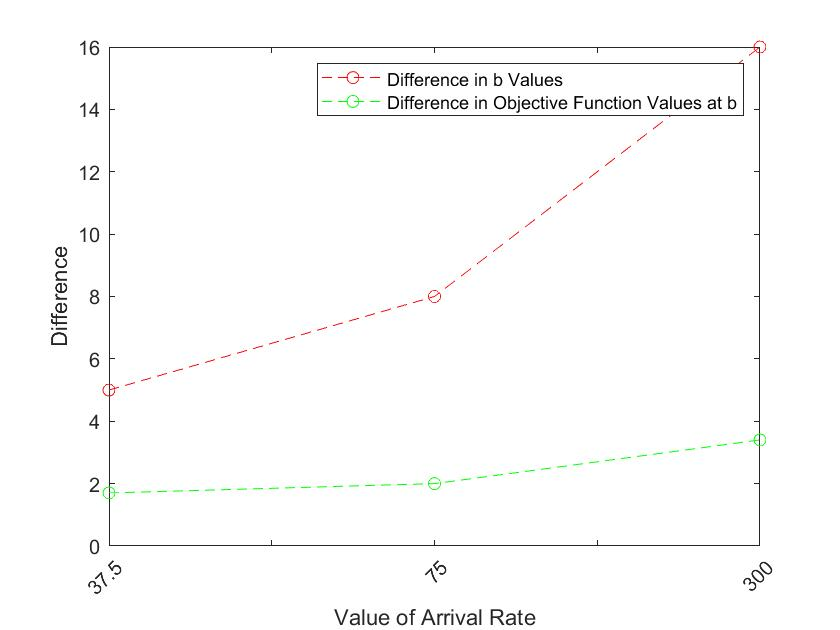
\includegraphics[height=7cm]{correctedDet.jpg}
\caption{Performance of the Proposed Solution on Deterministic Arrival Rates}
\end{figure}
\end{frame} 

\begin{frame}{Analysing the Performance of the Proposed Solution}
\textbf{Case II: Uncertain Arrival Rates} \\
We assume that the arrival rates follow a uniform distribution, U[a,b].
\[\bar{b}=F^{-1}(\frac{11}{12})= =\frac{11}{12}b-\frac{1}{12}a \]
\begin{table}
\small
            \begin{tabular}{|c||c|c|c|c|c|c|}
            \hline
            Arrival Rate &  \multicolumn{2}{|c|}{Optimal Solution} & \multicolumn{2}{|c|}{Proposed Solution}& \multicolumn{2}{|c|}{Comparison} \\
            \hline
                Distribution& $b^*$ & $\Pi(b^*)$ & $\bar{b}$& $\Pi(\bar{b})$& $|b^*-\bar{b}|$& Optimality Gap\\ 
                    \hline \hline
                    U[1,2] & 3 & 1.4 & 1 & 5.3 & 2& 3.8\\ 
                    U[2,4] & 5 & 2.2 & 3 & 3.3 & 2& 1.1\\
                    U[5,10] & 11 & 4.3 & 8 & 5.0 & 3& 0.7\\
                    U[10,20] & 20 & 7.7 & 17 & 8.0 & 3& 0.3\\
                    U[15,30] & 29 & 11.0 & 26 & 11.1 & 3& 0.2\\
                    U[20,40] & 37 & 14.2 & 35 & 14.3 & 2& 0.1\\
                    U[25,50] & 46 & 17.3 & 43 & 17.5 & 3& 0.2\\
                    U[50,100] & 89 & 33.1 & 87 & 33.2 & 2& 0.1\\
                    U[200,400] & 351 & 127.1 & 350 & 127.1 & 1& 0.0\\
            \hline
            \end{tabular} 
            \caption{Performance of the Proposed Solution on Uncertain Arrival Rates}            
\end{table}
The difference in the value of optimality gap in the two tables is quite high even though mean of arrival rate in the last 3 rows are same. This shows that the proposed solution works better when the arrival rate has uncertainty.
\end{frame} 

\begin{frame}{Analysing the Performance of the Proposed Solution}
\begin{figure}
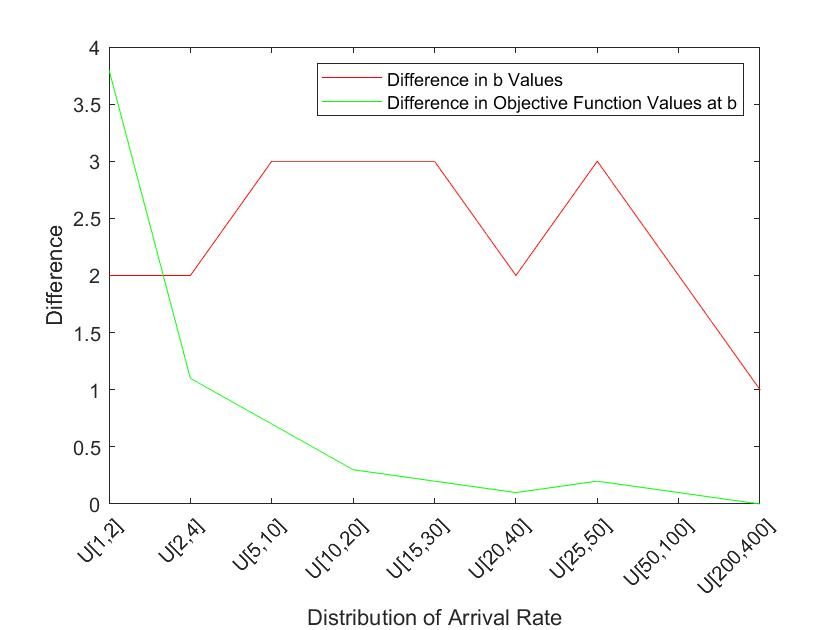
\includegraphics[height=7cm]{correctedUni.jpg}
\caption{Performance of the Proposed Solution on Uncertain Arrival Rates}
\end{figure}
\end{frame}
\section{Optimizing the system management cost in the presence of self scheduling }
\begin{frame}{Self scheduling Servers Background}
    So let us consider a multi period queuing model where the servers can self schedule whether to serve in a particular shift and the customers are impatient as in any real life system. \bigskip \\
    
    Let us consider a system with $k$ shifts and the queuing models for a individual shift to be 
$G/G/N_{j}^{n} +GI$ in steady state. Here , $N_{j}^{n}$ is a random variable that indicates the number of servers in $j^{th}$ shift which depends on the total number of servers $n$. We also assume that all the servers are identical and service are identically distributed independent random variables and they follow a general distribution with mean $\frac{1}{\mu}$ , and W.L.O.G , $\mu=1$ . Also there is no restriction on any server in successive shifts or multiple shifts.
\end{frame}
\begin{frame}{Modelling Framework}
    When the customer is waiting in the queue, after a random time, the customer leaves without being served, we call this time as patience time. Let us assume that the patience times are identically distributed independent random variables with a cdf $F$, complementary cdf ccdf $\bar{F}$, density function $f$, hazard-rate function $h_{a}$ and mean $\frac{1}{\theta}$. We assume the arrival, service, abandonment processes are mutually independent and also independent of the number of servers in a shift $N_{j}^{n}$. Also the queue is $FIFO$ and the capacity is unlimited. The customer arrival rate is stationary process of $\lambda_j$ for the $j^{th}$ shift.
\end{frame}
\begin{frame}{System Manager's Problem}
Being consistent with \textit{Bassamboo and Randhawa} , let's consider two costs in the system 
 \begin{itemize}
    \item a delay cost ${h_{j}}$ incurred per unit time a customer waits in the queue for being served in the $j^{th}$ shift
    \item a penalty ${p_{j}}$ incurred per every customer who abandons the system in the $j^{th}$ shift
\end{itemize}
Let $Q_{N_{j}^{n}}$ be the queue length and $\alpha_{N_{j}^{n}}$ be the net abandonment. The system manager can decide on the staffing level $n$ , the problem becomes
\begin{equation}
   \min_{n \in \mathbb{N}} \Pi(n) = \sum_{1 \leq j \leq k} ({c_{j}\mathbb{E}[N_{j}^{n}]+p_{j}\mathbb{E}[\alpha_{N_{j}^{n}}]}+h_{j}\mathbb{E}[Q_{N_{j}^{n}}])   
\end{equation}
where $c_j$ is the compensation for each server in $j^{th}$ shift.
\end{frame}
\begin{frame}{Fluid Approximation of System Manager's Problem}
Since an exact analysis of (1) is difficult, let us consider a fluid approximation of the above problem, we will later show that the fluid approximation works good in case of a binomial distribution for the number of servers. 
\\ "For an $G/G/s +GI$ system, $\bar{q}_{\rho_{s}}$ and $\bar{\alpha}_{\rho_{s}}$ are the fluid approximations of queue length and net abandonment rates respectively, with traffic intensity $\rho_{s} \equiv \frac{\lambda}{\mu s}$. This result is obtained from \textit{Whitt(2006)}"
\\ So the fluid approximation for (1) is
\begin{equation}
    \min_{n \in \mathbb{N}} \Pi(n) = \sum_{1 \leq j \leq k} {n G(c_j)c_j+p_j.\bar{\alpha}_{{\rho_{s}}/{G(c_j)}}+h_j.\bar{q}_{{\rho_{s}}/{G(c_j)}}}
\end{equation}
Here, $\mathbb{E}[N_{j}^{n}] = G(c_j)$ , since $G(c_j)$ is a constant , let it be $r_j$ , which we define as availability of a server in $j^{th}$ shift. In the fluid approximation, we can see that the optimal staffing level is only dependent on the expectation of the number of servers in a particular shift , but in reality , the variance is a important factor as well which we will discuss later in the paper.
\end{frame}
\begin{frame}{Benchmark case : No self scheduling}
    Before we proceed to the problem, let us take a benchmark case where there is no self scheduling which means $r_j$=1 , for all the shifts.\\ The queue length in $j^{th}$ shift can be written as 
 \begin{equation}
     q_j = \int_{0}^{w_j} \lambda_j \bar{F}(u)  \, du
 \end{equation}
  The net abandonment rate in $j^{th}$  shift can be written as
  \begin{equation}
      \alpha_j=\lambda_j F(w_j)
  \end{equation}
   where $w_j$ denotes the waiting time in given shift $j$.
 Clearly, when there is no self-scheduling the individual optimal staffing in each shift 
 \begin{equation}
     n_j^{*}=\lambda \bar{F}(w_j^{*})
 \end{equation}
  where $w_j^{*}$ would be the optimal waiting time.
\\With the results in (5) and (4) the system managers problem becomes
\begin{equation}
    min_{w_j \geq 0} \left( \lambda_j c_j \bar{F}(w_j) - \lambda_j p_j \bar{F}(w_j) + \lambda_j h_j\int_{0}^{w_j} \lambda_j \bar{F}(u)  \, du \right)
\end{equation}
\end{frame}
\begin{frame}{Some results for the bench marking case}
    \textbf{ Assumption} $For$ $all$ $j$ , $c_j$ $<$ min($h_j/h_a(0)+p_j,h_j/\theta+p_j$)
\\ The above assumption tells us that this source of servers are economical enough for the manager to staff from them and not avoid them altogether, this is consistent with the assumption in Bassamboo , also if the abandonment process is exponential , we have $h_a(t) = \theta t$ , so $h_a(0) =0$ , the first term becomes $\inf$ , so the assumption becomes
\begin{equation}
    c_j < h_j/\theta +p_j
\end{equation}
Using this , we will try and show the next proposition 
\\\textbf{Proposition} \textit {Under the above assumption , to optimise the costs in a system with no self scheduling , we should load all the shifts critically} , $i.e.$ $n_j^{*}=\lambda_j$ for all $j$
\end{frame}
\begin{frame}{Servers with Self- Scheduling capability}
     In this case , the $r_j$ factor is no longer $1$, so we define a new arrival rate called the \textit{augmented arrival rate} $\Gamma_j$.
 The augmented arrival rate is defined as the ratio of actual arrival rate and the showup probability $i.e$ $\Gamma_j = \lambda_j/r_j$
  \\Also W.L.O.G , we will assume that the shifts are ordered in the increasing order of $\Gamma_j$
 $i.e$ $\Gamma_{j-1} \leq \Gamma_{j}$ for $j$={$1,2,...,k$}
 \\so the system manager's problem in terms of the augmented arrival rate $\Gamma_j$ becomes 
\begin{equation}
      min_{0 \leq n \leq \Gamma_k} C(n) = \left( \sum_{j=1}^{k} {I(\Gamma_{j-1}\leq n <\Gamma_j)u_j(n)}\right)
\end{equation}
where $I(n \in S)$ is a indicator random variable that tells us whether the value $n$ is in the set $S$ and $u_j(n)$ is given by 
\begin{equation}
u_j(n)=\sum_{i=1}^{k}{c_inr_i}+\sum_{i=j}^{k}{\left ( p_i( \lambda_i-nr_i)+ h_i\lambda_i \int_{0}^{\bar{F}^{-1}(n/\Gamma_i)}  \bar{F}(u)  \, du \right)}
\end{equation}
this $u_j$ represents the cost of the system if $n$ is chosen in the [$\Gamma_{j-1}$,$\Gamma_j$), also we can see that only one of the indicator variables is non-zero and the rest of them are zero.
\end{frame}
\begin{frame}{Some results for self scheduling case}
    \textbf{Proposition 3.2.} \textit{If the calculated $\Gamma_j$ ("resulting augmented arrival rates") are equal across all shifts then and only then, the self scheduling system is not more expensive than a system with no self scheduling}
    \begin{proof} \label{}
Let all the augmented arrival rates be equal $i.e$ $\Gamma_j=\Gamma$, then assuming that $n^{*}=\Gamma$ gives, $n_i^{*}=n^{*}r_i=\lambda_i$ for all shifts, as we have seen in proposition int the benchmark case, this is the optimal staffing cost in the case of the benchmark, so if all the augmented arrival rates are equal , we can eliminate the cost of self scheduling. 
\end{proof}
\end{frame}
\begin{frame}{Some results for self scheduling case}
 \textbf{In case of Exponential Abandonment and Non-equal Augmented Arrival Rates:}
 \\\textit{
\begin{enumerate}
    \item The optimization function in (8) is piece-wise linear.
    \item There exists one shift $s$, such that by matching the demand in that shift we can optimize the system $i.e.$ $n^{*}=\Gamma_{s}$.
    \item $i_0$ satisfies the following condition:
    \begin{equation}
        \sum_{j=1}^{k}c_jr_j-\sum_{j=i_0}^{k}\left(p_j+h_j/\theta \right)r_j < 0\,\,and
        \sum_{j=1}^{k}c_jr_j-\sum_{j=i_0+1}^{k}\left(p_j+h_j/\theta \right)r_j > 0
    \end{equation}
\end{enumerate}}
\end{frame}
\section{Future Steps...}
\begin{frame}{Future Steps ...}
    In the coming semester , we would try to combine the both parameter uncertainty and self scheduler servers and arrive at a optimal staffing for the queuing system taking the $Dong\,and\,Ibrahim$ paper, also try to introduce a new worker $freelancer$ as an extension to that model and look at the fluid approximations considered in this paper, and see if we can forgo them.
\end{frame}
\end{document}